\section{Results}
\subsection{Calibration}
Due to the construction and hardware of the antenna, the pointing of the antenna doesn't always line up with the target. It is therefore necessary to calibrate it before pointing at distant objects. The Sun being the strongest discrete radio source in the sky \cite{burke_introduction_2013}, mostly due to black body radiation.
By configuring the antenna to point towards Sun, using its actual coordinates, and scanning the surrounding area in Az/Alt coordinates, the maximum average measured power gives the real position of the Sun in the specific antenna coordinates. The measured power and a linear interpolation of those values shown in \autoref{fig:calibration_contour} gives a correction of
\begin{equation}
    \textrm{Az: } -5^\circ \qquad \textrm{Alt: } -2^\circ \\
    \textrm{PLEASE EXECUTE THE NOTEBOOK EXP1 WITH UNCOMMENTED THING IN contourf\_az\_alt}
\end{equation}


\hl{OLD STUFF}
\hl{Details d'où vient le signal etc}.
The first preliminary measures indicated a maximum of the signal power a point to the bottom left of the sun.
Therefore a series of measures were made in order to draw a grid to the bottom left of the sun. The position of the sun was recorded for each measure in order to study the relative position.
By interpolating the obtained values of power, the contour map depicted in \autoref{fig:calibration_contour} was obtained.

[aussi \cite{lauterbach_radio_2022} parle du soleil, section 4.1]

\begin{figure}[htbp]
    \centering
    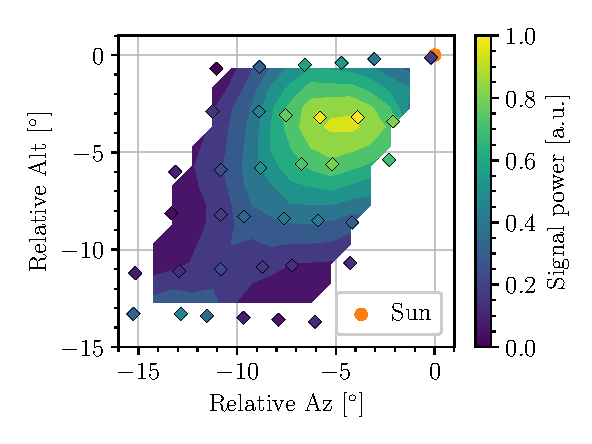
\includegraphics[scale=1]{figures/calibration_contour.pdf}
    \caption{Calibration contour}
    \label{fig:calibration_contour}
\end{figure}

\subsection{Distinguishing signal and noise}
Measure BM building, measure actual H21 source, divide actual by noise to extract the signal from noise, apply some filter and voilà, a nice signal

\subsection{Velocity field of the Milky Way}
Probing arms of milky way

Talk about orientation (i.e. sky visible at measuring time), correct angular momentum?
